\documentclass{article}
\usepackage{natbib}

\usepackage{graphicx}
\usepackage{url}

\title{Supplementary Material for tstrait: a quantitative trait simulator for ancestral recombination graphs}
\date{}
\usepackage[margin=1in]{geometry}

\begin{document}
\maketitle

\section{Supplementary Notes}

We present an overview of statistical tests that are conducted during the development process of the \texttt{tstrait} package. Three types of tests are conducted to validate the statistical properties of \texttt{tstrait}: exact tests, comparison tests, and statistical tests.

\subsection{Exact Tests}

We simulate effect sizes and phenotypes without environmental noise by using two different quantitative trait simulators, \texttt{AlphaSimR}~\citep{gaynor2021} and
\texttt{simplePHENOTYPES}~\citep{fernandes2020}, and the simulation framework described in \citep{zhang2023}. The simulated effect sizes are directly used in \texttt{tstrait} to simulate phenotypes. We show that when traits are influenced with the same causal sites and effect sizes, the simulated genetic values from \texttt{tstrait} are identical to the other simulation frameworks.

\subsection{Comparison Tests}

We simulate phenotypes with environmental noise in \texttt{AlphaSimR}~\citep{gaynor2021},
\texttt{simplePHENOTYPES}~\citep{fernandes2020} and the simulation framework described in \citep{zhang2023} by using the same parameters that are used in the \texttt{tstrait} simulation. By using QQ-plots, we show that the simulated traits from \texttt{tstrait} are having similar distributions as the traits simulated from other programs.

\subsection{Statistical Tests}

Environmental noise and effect sizes are simulated by using various parameters in \texttt{tstrait} and their statistical properties are validated by using QQ-pplots.

\subsection{Availability of Materials}

Code to run the statistical tests is included in the \texttt{tstrait} GitHub repository, \url{https://github.com/tskit-dev/tstrait/blob/main/verification.py}. These tests are used as part of the development process of the \texttt{tstrait} package.

\section{Supplementary Figures}

\renewcommand\thefigure{S\arabic{figure}}
\setcounter{figure}{0}
\renewcommand\thetable{S\arabic{table}}
\setcounter{table}{0}

\begin{figure}[h]%
\centering
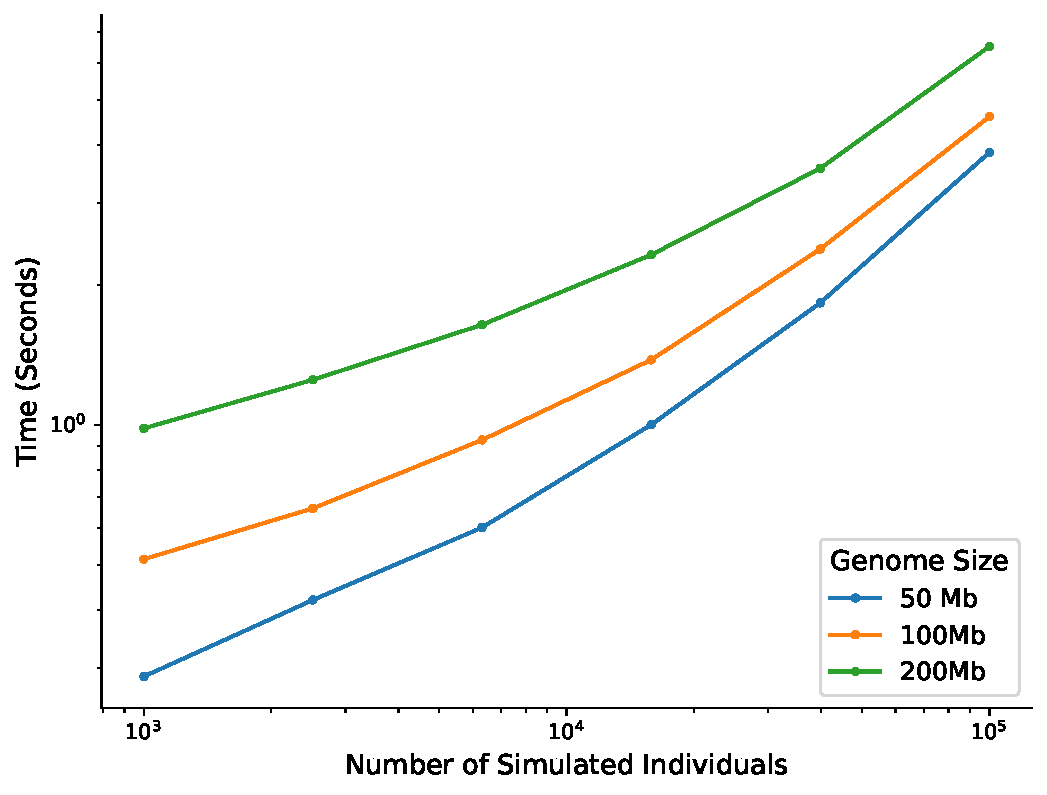
\includegraphics[width=0.7\columnwidth]{figures/stdpopsim-time.pdf}
\caption{Time taken to simulate quantitative traits with increasing
sample size. For each sample size, we simulated an ARG under human-like
parameters using the default HomSap demographic model in \texttt{stdpopsim}.
Each point represents the mean time for 10 independent runs of \texttt{tstrait}
for a particular ARG. The times reported are the total CPU
time required to simulate a quantitative trait with 1000 causal sites,
on an Intel(R) Core(TM) i9-11900H CPU and 16 GB of RAM.
The trait model is a normal distribution with $\mu=0$,
$\sigma^2=1$, $h^2=0.3$, and $\alpha=0$.
}\label{fig:time}
\end{figure}

\newpage

\bibliographystyle{abbrvnat}
\bibliography{paper}

\end{document}